\chapter{System Design}

The software design describes the final details of a system before it is implemented. During the design process decisions are taken in order to meet the gathered requirements, decisions that are then applied to the system defined in the section Specification 3. Both physical and logical designs of the system are described in detail in the current chapter (sections System Physical Architecture 4.1 and System Logical Architecture 4.2), with an overview of how the resulting product needs to be implemented. Every technology used is carefully justified and the major characteristics are explained (section Description of Used Technologies).

The selection of a technology is a decisive process aimed to obtain the optimal results of a project. An unwise decision can sometimes seriously affect the total resources needed or the successful fulfillment of the proposed objectives. It is also important to design correctly the structure of the system, for example identifying and applying the software patterns that can solve existing problems in this particular project.

\section{Design Class Diagram}

\subsection{Class Diagram Description}
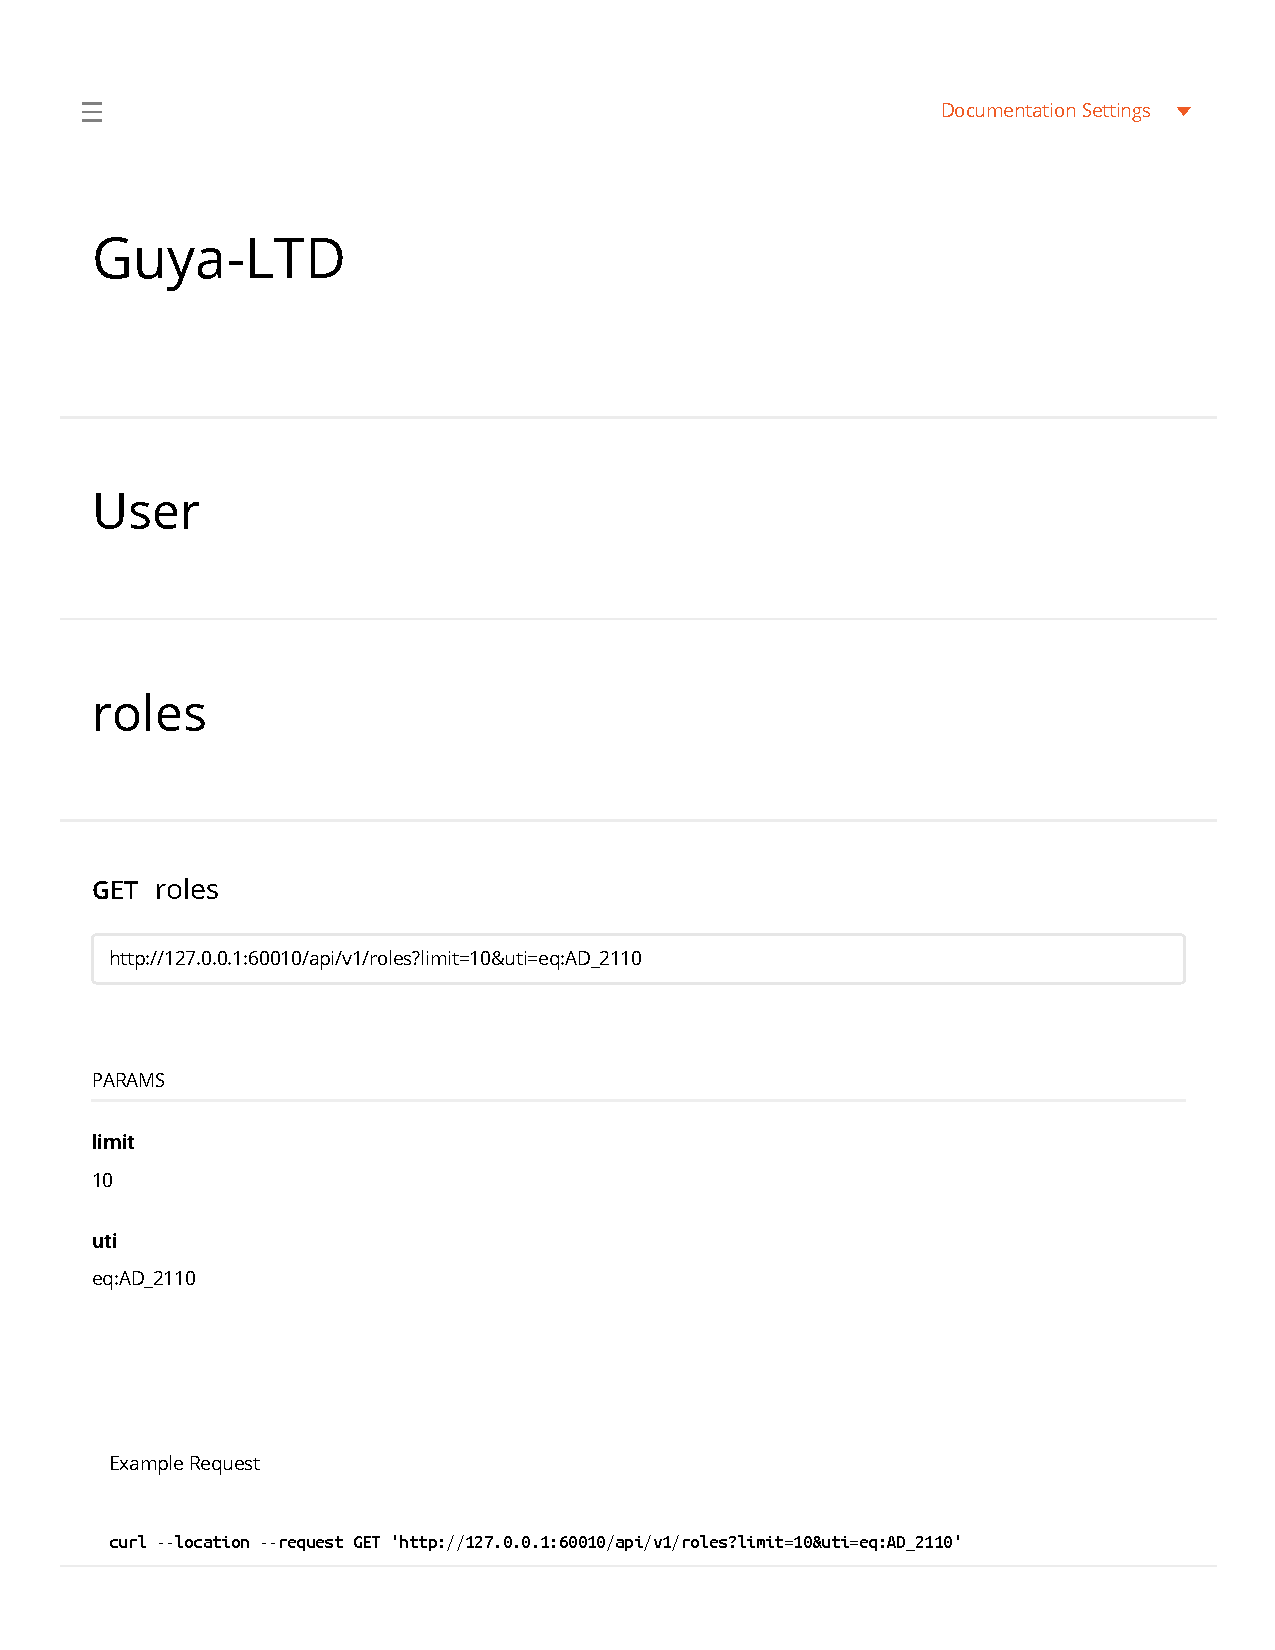
\includepdf[page=-, pagecommand={}]{pdf/Guya-LTD-api.pdf}

\section{Database Design}
%\subsection{Normalization}

\subsection{Physical Data Model}
\begin{figure}[!h]
%\hspace{-3cm}
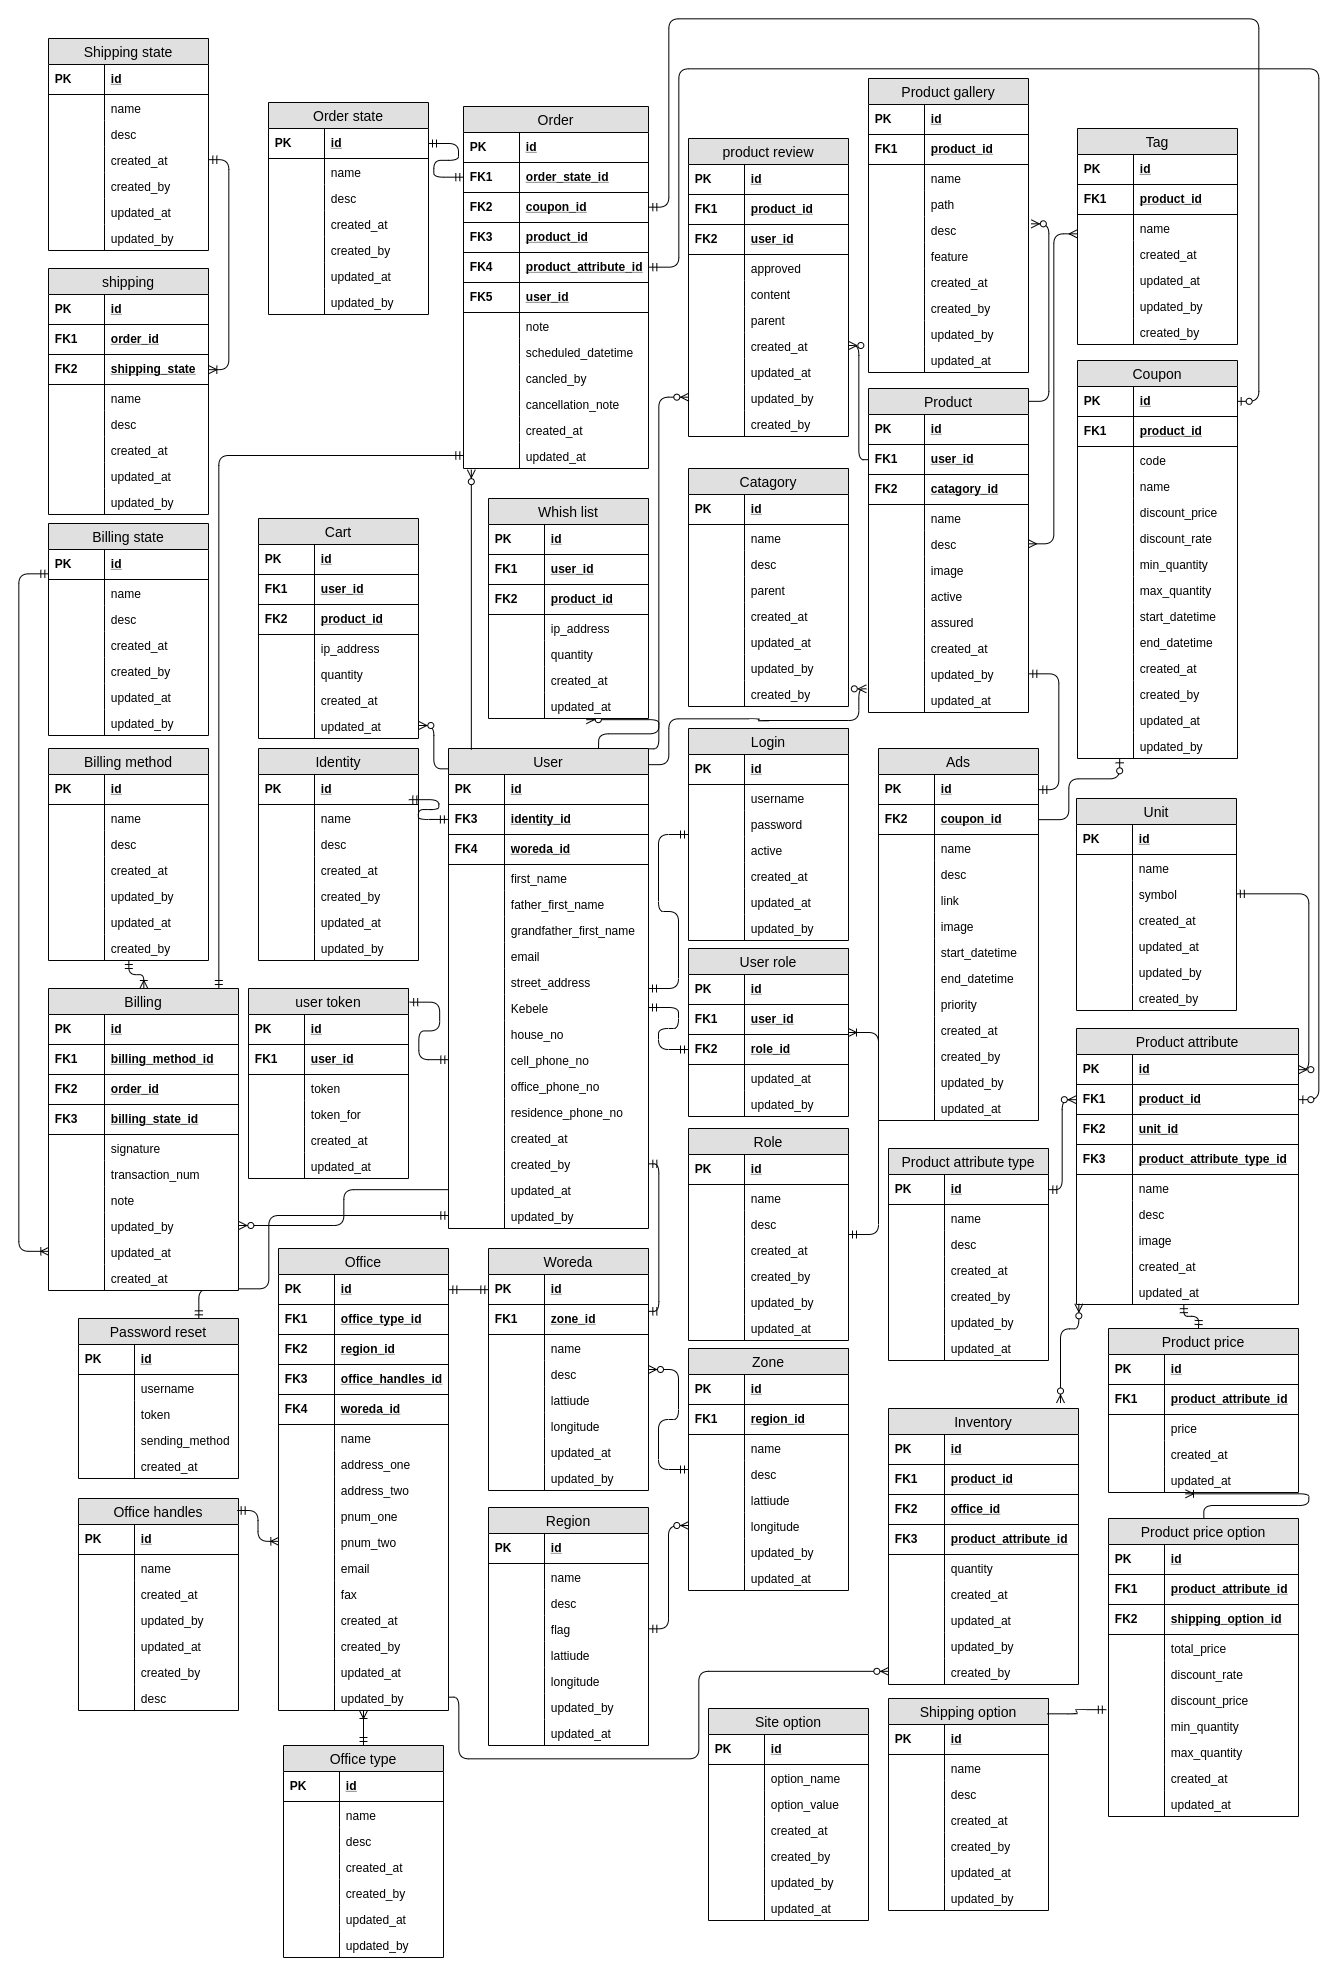
\includegraphics[width=17cm, keepaspectratio]{usecases/shop_database_diagram}
\caption{Physical data model - Guya E-commerce}
\end{figure}
\clearpage

\begin{figure}[!h]
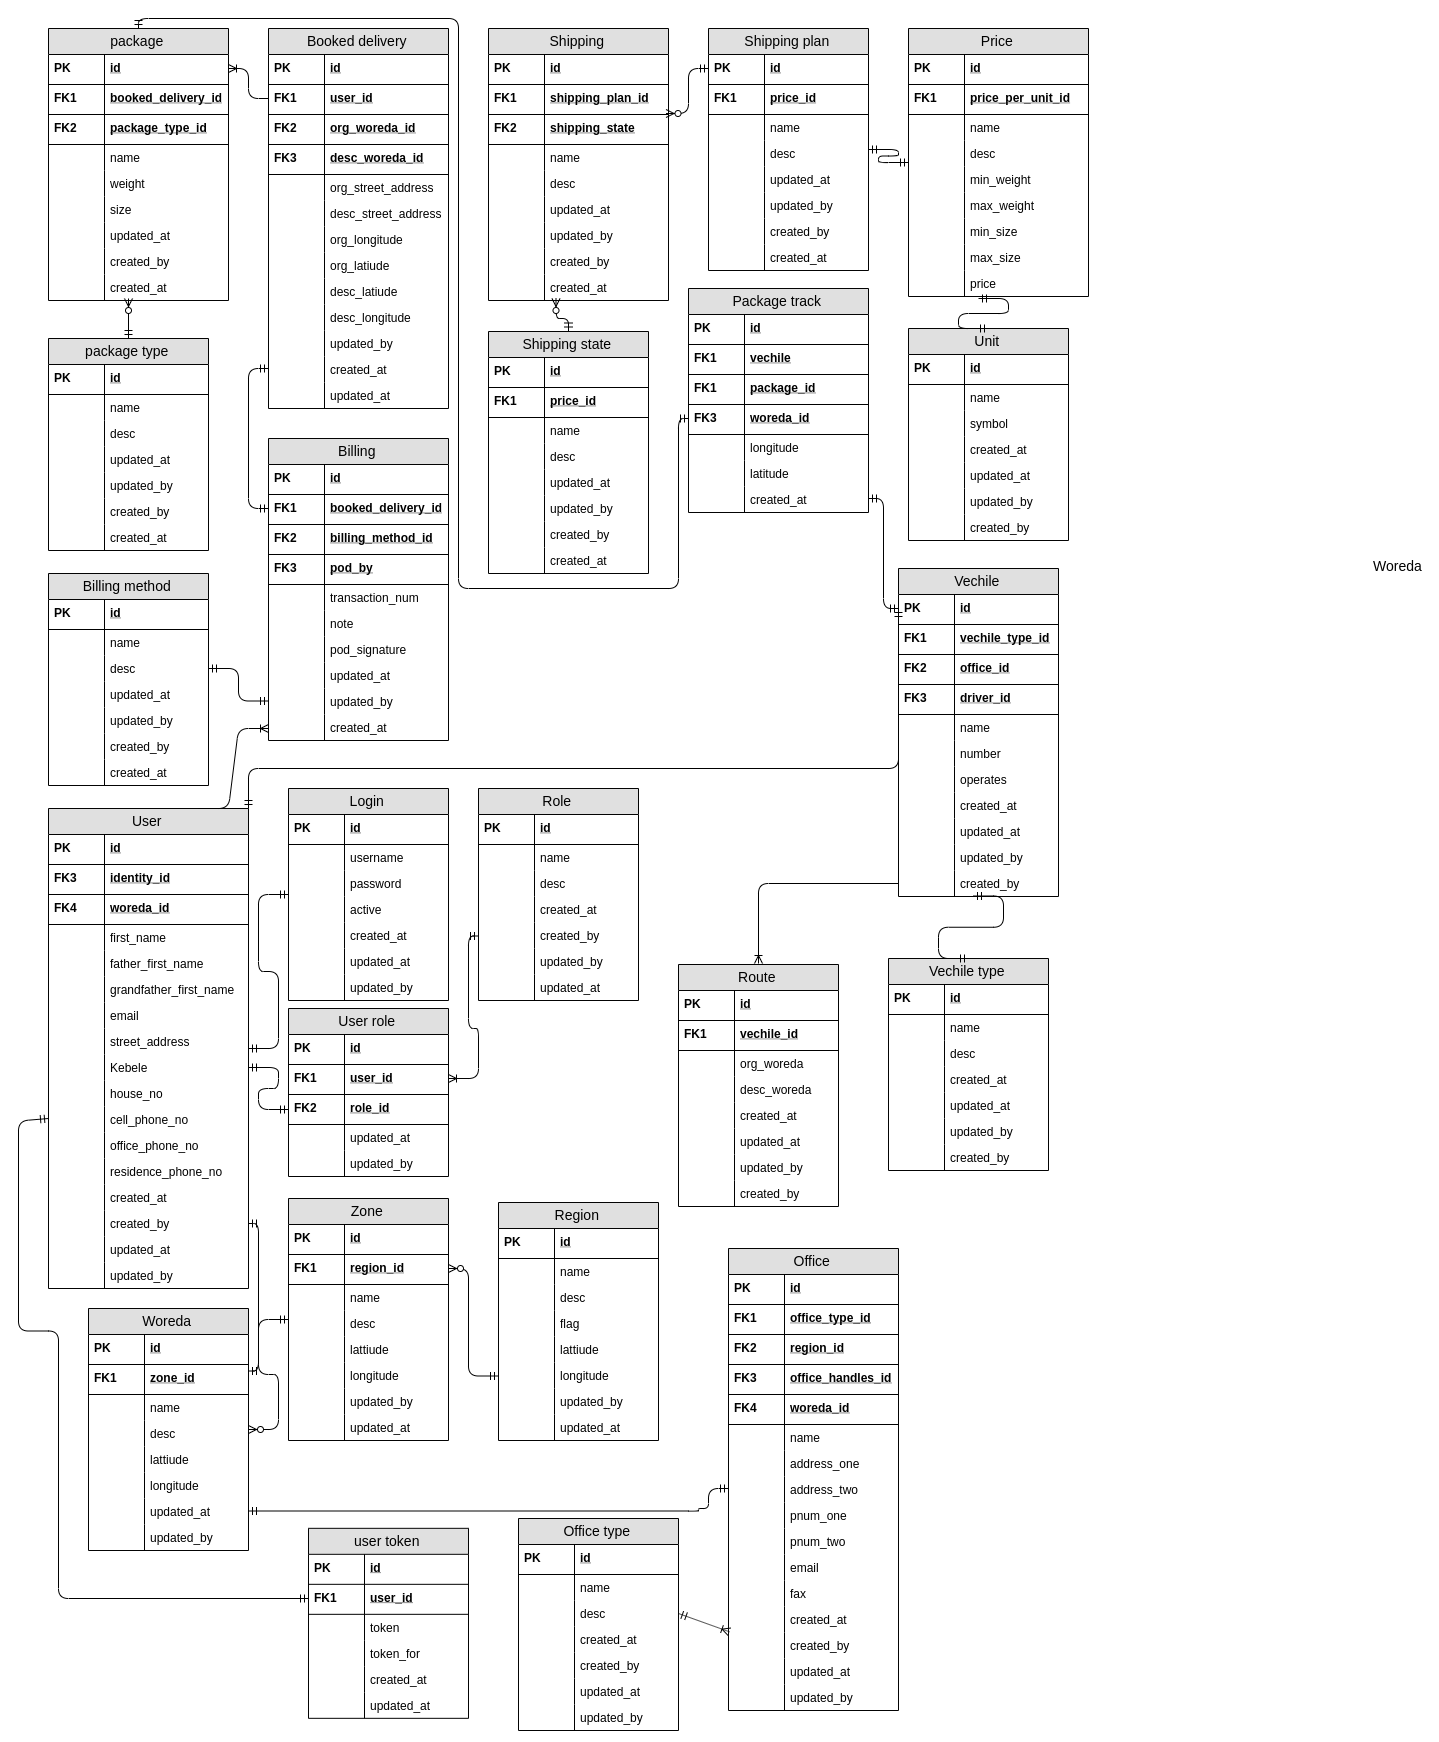
\includegraphics[width=20cm, keepaspectratio]{images/xpress_database_diagram}
\caption{Physical data model - Guya E-commerce}
\end{figure}
\clearpage


\section{User Interface Design}
Undoubtedly, it is difficult to imagine how a new system will look and behave from reading a textual requirements specification. There are three ways to visualize textual requirements:
\begin{description}
	\item[Wireframes:] are schematic pages used as a visual guide that shows the pilot system framework. They aim to represent functionality without displaying Visual elements.
	\item[Mockups:] reflect the design choices for color schemes, layouts, typography, iconography, the visuals of navigation, and the overall system design solutions; are static and unclickable.
	\item[Prototypes:] are clickable system representations that display how users can interact with the system in a real world; enable designers to test users journey and find potential issues throughout the interaction flow.
\end{description}

\subsection{Website Wierframe Visual Guides}
A website wireframe, also known as a page schematic or screen blueprint, is a visual guide that represents the skeletal framework of a website. Wireframes are created for the purpose of arranging elements to best accomplish a particular purpose. The purpose is usually being informed by a business objective and a creative idea. The wireframe depicts the page layout or arrangement of the website's content, including interface elements and navigational systems, and how they work together. The wireframe usually lacks typographic style, color, or graphics, since the main focus lies in functionality, behavior, and priority of content. In other words, it focuses on what a screen does, not what it looks like. Wireframes can be pencil drawings or sketches on a whiteboard, or they can be produced by means of a broad array of free or commercial software applications, the type of software application we used to sketch the diagrams is stated in subsection \ref{software_requirements}. Wireframes are generally created by business analysts, user experience designers, developers, visual designers, and by those with expertise in interaction design, information architecture and user research, but in our case; since it is a Capstone project we do not have a labor division only concerned with user interface design. Below are wireframe figures for both websites.

\subsubsection{Display Products}
Product listing is the first functionality that a customer uses when arriving at the web-shop and the one he will be using for longer periods of time, so it needs to have a comfortable way to display and paginate the products. At best, traditional web-shops usually have very rigid ways of listing products: pagination consists of an interface that allows to select the page and the amount of products per page, while display options let the user select between a list or a grid type of view.

So instead of showing a traditional shop catalog, it was considered a better option to let the products flow freely through the web page, using all the width and height possible to show at once the maximum amount of products to the user (Figure \ref{display-products}). On the other hand, the pagination needs to be natural without losing already viewed products, so when the user reaches the bottom of the page new products should appear automatically under the previous ones.

The product thumbnails, besides price and name, will be showing a picture of the product and the different color variants. The selected variant will be highlighted, and when hovering a different color the thumbnail will be updated with that variant information, such as picture and price, if different. The thumbnail will also include a button to add the selected product variant to the shopping cart. In case the product has different sizes available, when hovering the button a list of the different sizes will be shown, so that the user can select the desired size he wants to add to the cart.

\begin{figure}[!h]
\center
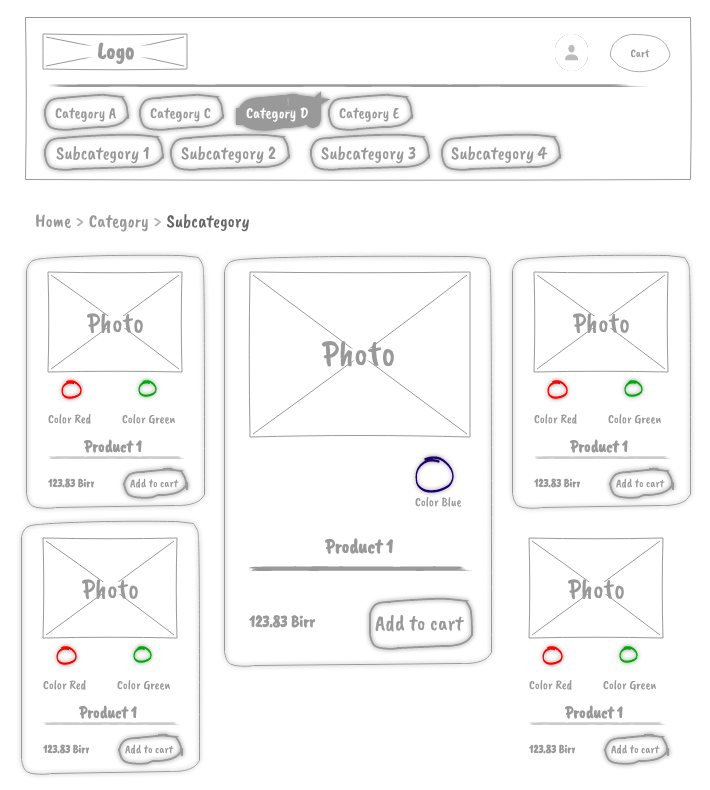
\includegraphics[keepaspectratio, width=15cm]{wireframes/productlist.png}
\caption{Wireframe prototype of the product listing screen, filtering by category - Guya E-commerce}
\label{display-products}
\end{figure}

When clicking on a product thumbnail the user will be redirected to the product detail of the variant he had selected (Figure \ref{product-detail}), if any. There he can select any other color variant, in which case a new page will be loaded in order to update the URL, to let the user share the product URL that points to this particular color. He can also select a different size, but in this case the page is not reloading, as it was considered that the user does not have a need to share the exact size. Below one can add the selected product variant to the cart, optionally indicating the exact quantity.

\begin{figure}[!h]
\center
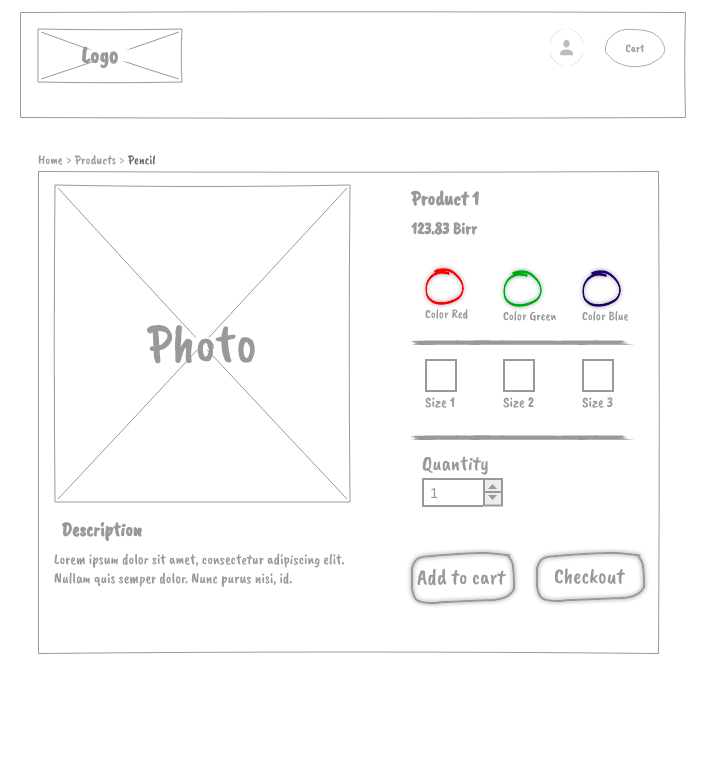
\includegraphics[keepaspectratio, width=15cm]{wireframes/product-detail.png}
\caption{Wireframe prototype of the product detail screen - Guya E-commerce}
\label{product-detail}
\end{figure}
\clearpage

The header contains a mini-cart and the login panel throughout the website. In any product list or product detail page, the header also contains the categories and subcategories of the shop to let the user filter products by category. The rest of the pages should contain a button to allow the user go back to the last category or product he visited. When scrolling, the header is always kept at the top of the page. Below the header, a breadcrumb is showing the current category path.

Whenever a product is added to the cart, the mini-cart located on the header appears for a few seconds, to let the customer know that the product was added successfully. At any time the user can see again the contents of his shopping cart when hovering the cart button on the header, that will be closed automatically when moving the cursor away from the mini-cart.

\subsubsection{Purchase products}

In order to start the checkout process, the user will first access the cart detail page by clicking on the cart button. This page shows the items and their details, along with the possibility to remove them or change the number of units of each item (Figure \ref{shopping-cart}). Both actions are performed without reloading the page, just updating the contents of the shopping cart and the pricing details accordingly.

\begin{figure}[!h]
\center
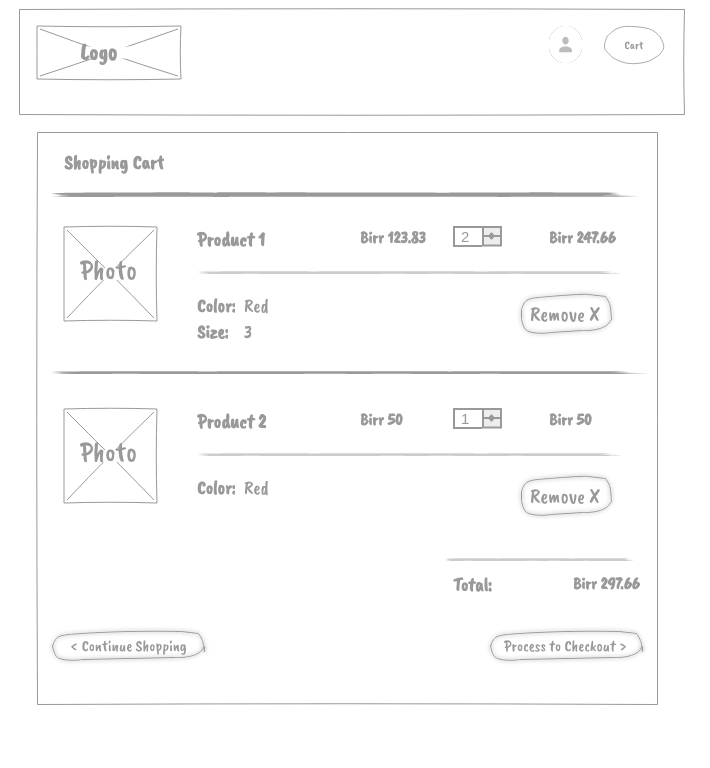
\includegraphics[keepaspectratio, width=15cm]{wireframes/shoppingcart.png}
\caption{Wireframe prototype of the shopping cart detail screen - Guya E-commerce}
\label{shopping-cart}
\end{figure}
\clearpage

The checkout page can be accessed from both mini-cart and cart detail page. The checkout page is probably one of the least frequented pages of a web-shop, but it is for sure the most important when it comes to user experience. The customer needs to feel he has control of the flow and that he is able to quit at any time. The checkout needs to be a secure and robust environment to the user.

Traditional web-shops usually reload when moving from one checkout step to the other, and it can be sometimes difficult to change the data of a step that is not immediately before the active one. In some cases it is also hard to know what changes are modifying the price or to review what was entered on previous steps. All these issues are affecting negatively the feeling of control the user has.

\begin{figure}[!h]
\center
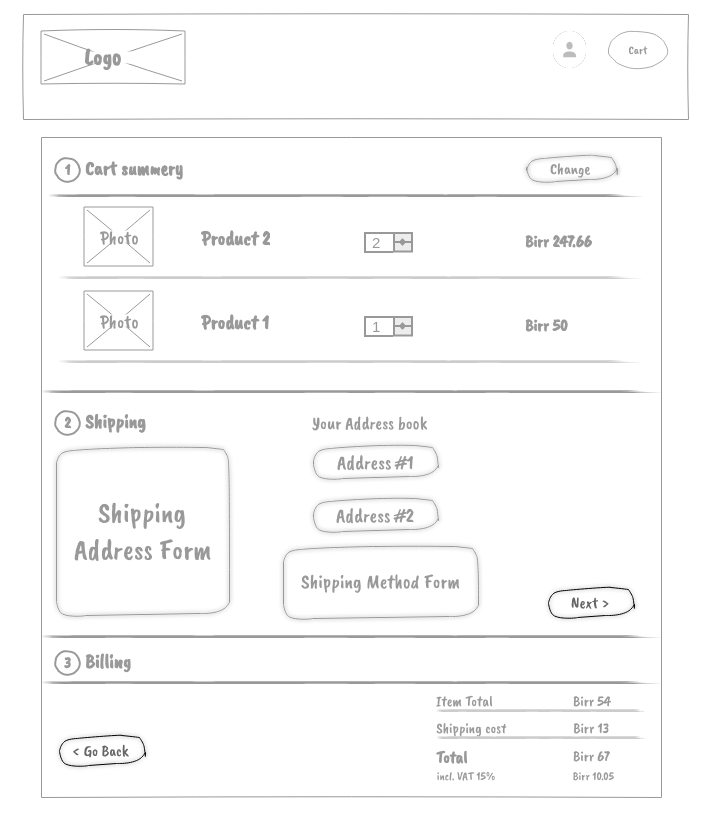
\includegraphics[keepaspectratio, width=15cm]{wireframes/checkoutpage.png}
\caption{Wireframe prototype of the shopping cart detail screen - Guya E-commerce}
\label{checkout-page}
\end{figure}
\clearpage

For this design it was considered a good idea to display all the steps throughout the page as sections that can be expanded, so that the user modifies them (see Figure \ref{checkout-page}). Once edited, the section closes again and displays a summary with the selected options. Every change automatically updates the pricing details that are always shown at the bottom of the page. As a way of guiding the customer through the checkout process, the user can only open new sections sequentially. Also when a form is still not available due to missing requirements (e.g. shipping method cannot be displayed until shipping address is set) a message will be shown instead until the requirements are met.
The checkout is divided into three steps: first a cart summary, to verify the items are correct; second the shipping information, to determine where and how the goods are being delivered; and third the billing information, to select the way the products are being paid. Both shipping and billing sections have on the left side a form to set the postal address and on the right side the shipping and payment options, respectively. When the customer is logged in, his address book will appear on the right side, allowing him to select one of his addresses, which data will then be copied to the corresponding address form.


\subsubsection{User Management}
Before attempting to access his profile page, the user needs to identify himself to the system. This is done in the login screen, a page that also contains a form to register into the system (see Figure \ref{login-page}). In case the user forgot his password, the login form contains an option to recover it, which renders a modal window where an email address is requested when the option is clicked.

\begin{figure}[!h]
\center
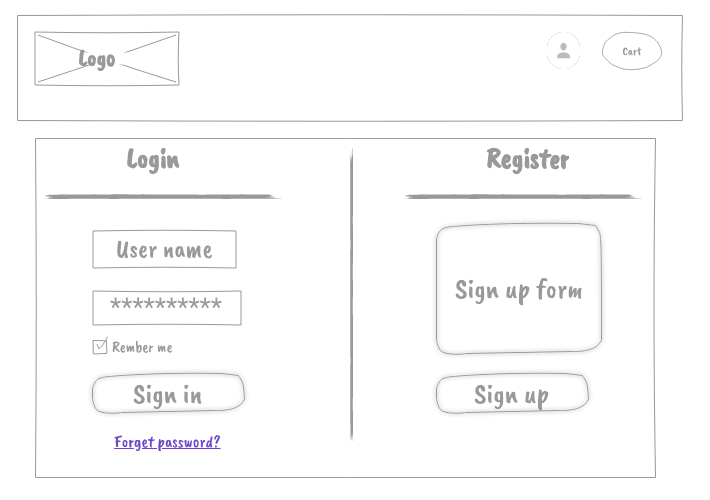
\includegraphics[keepaspectratio, width=15cm]{wireframes/loginpage.png}
\caption{Wireframe prototype of the login screen - Guya E-commerce and Express}
\label{login-page}
\end{figure}
\clearpage

Submitting this form will send an email to the user with a new URL, that redirects to the same login page but with a different modal window to enter a new password. Once the password is submitted the modal window closes, thus showing the login form again to allow the user enter his new credentials.

\begin{figure}[!h]
\center
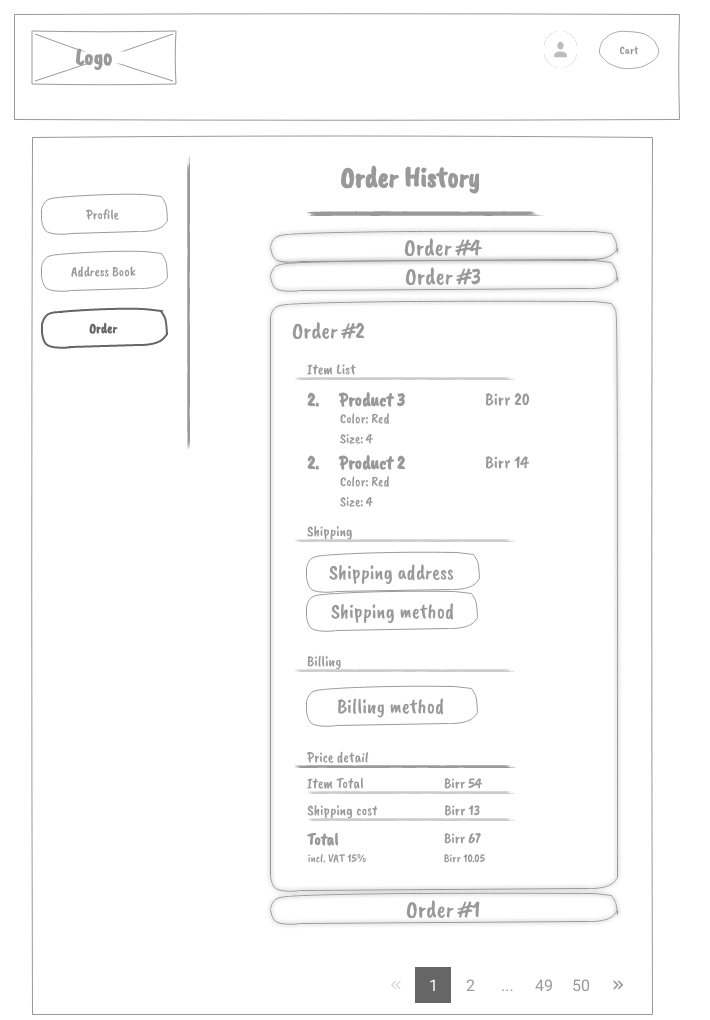
\includegraphics[keepaspectratio, width=15cm]{wireframes/orderlist.png}
\caption{Wireframe prototype of the user profile screen, order list section - Guya E-commerce}
\label{order-list}
\end{figure}
\clearpage

The user profile is a single page with sections to change user data, password, manage the address book and view the list of orders (see Figure \ref{order-list}). The latter consists of some stockable sections, each one containing all information about a particular order, such as the products purchased, the price details and all shipping and billing related information. When clicking on a section, this one expands showing its contents, while all other sections remain closed.

\begin{figure}[!h]
\center
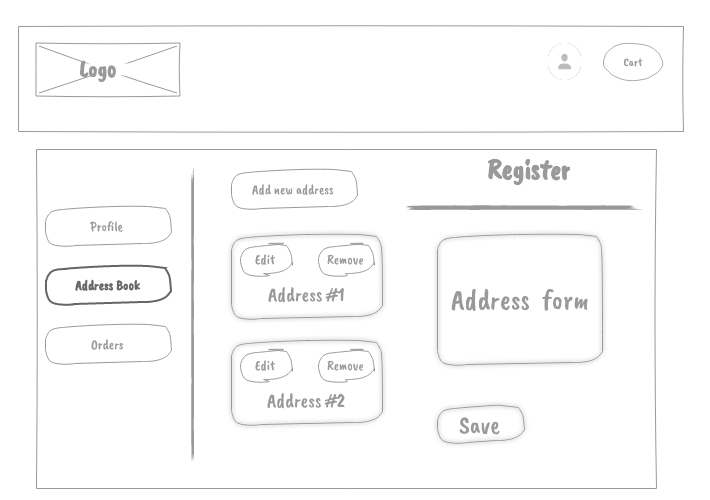
\includegraphics[keepaspectratio, width=15cm]{wireframes/customeraddressbook.png}
\caption{Wireframe prototype of the user profile screen, address book section - Guya E-commerce}
\label{addressbook-section}
\end{figure}
\clearpage

The address book is the only section with a slightly complex design. This component has a list of existing addresses on the left and an empty form on the right to add a new address (Figure \ref{addressbook-section}). When the user selects an address the form changes into edition mode, highlighting the address and copying its data to the empty form. A button at the top allows the user to return the form to its initial mode. Whenever the user adds, updates or removes an address, the list of addresses is updated accordingly.


\subsection{Mail Interface Templates}

\clearpage
\begin{figure}[!h]
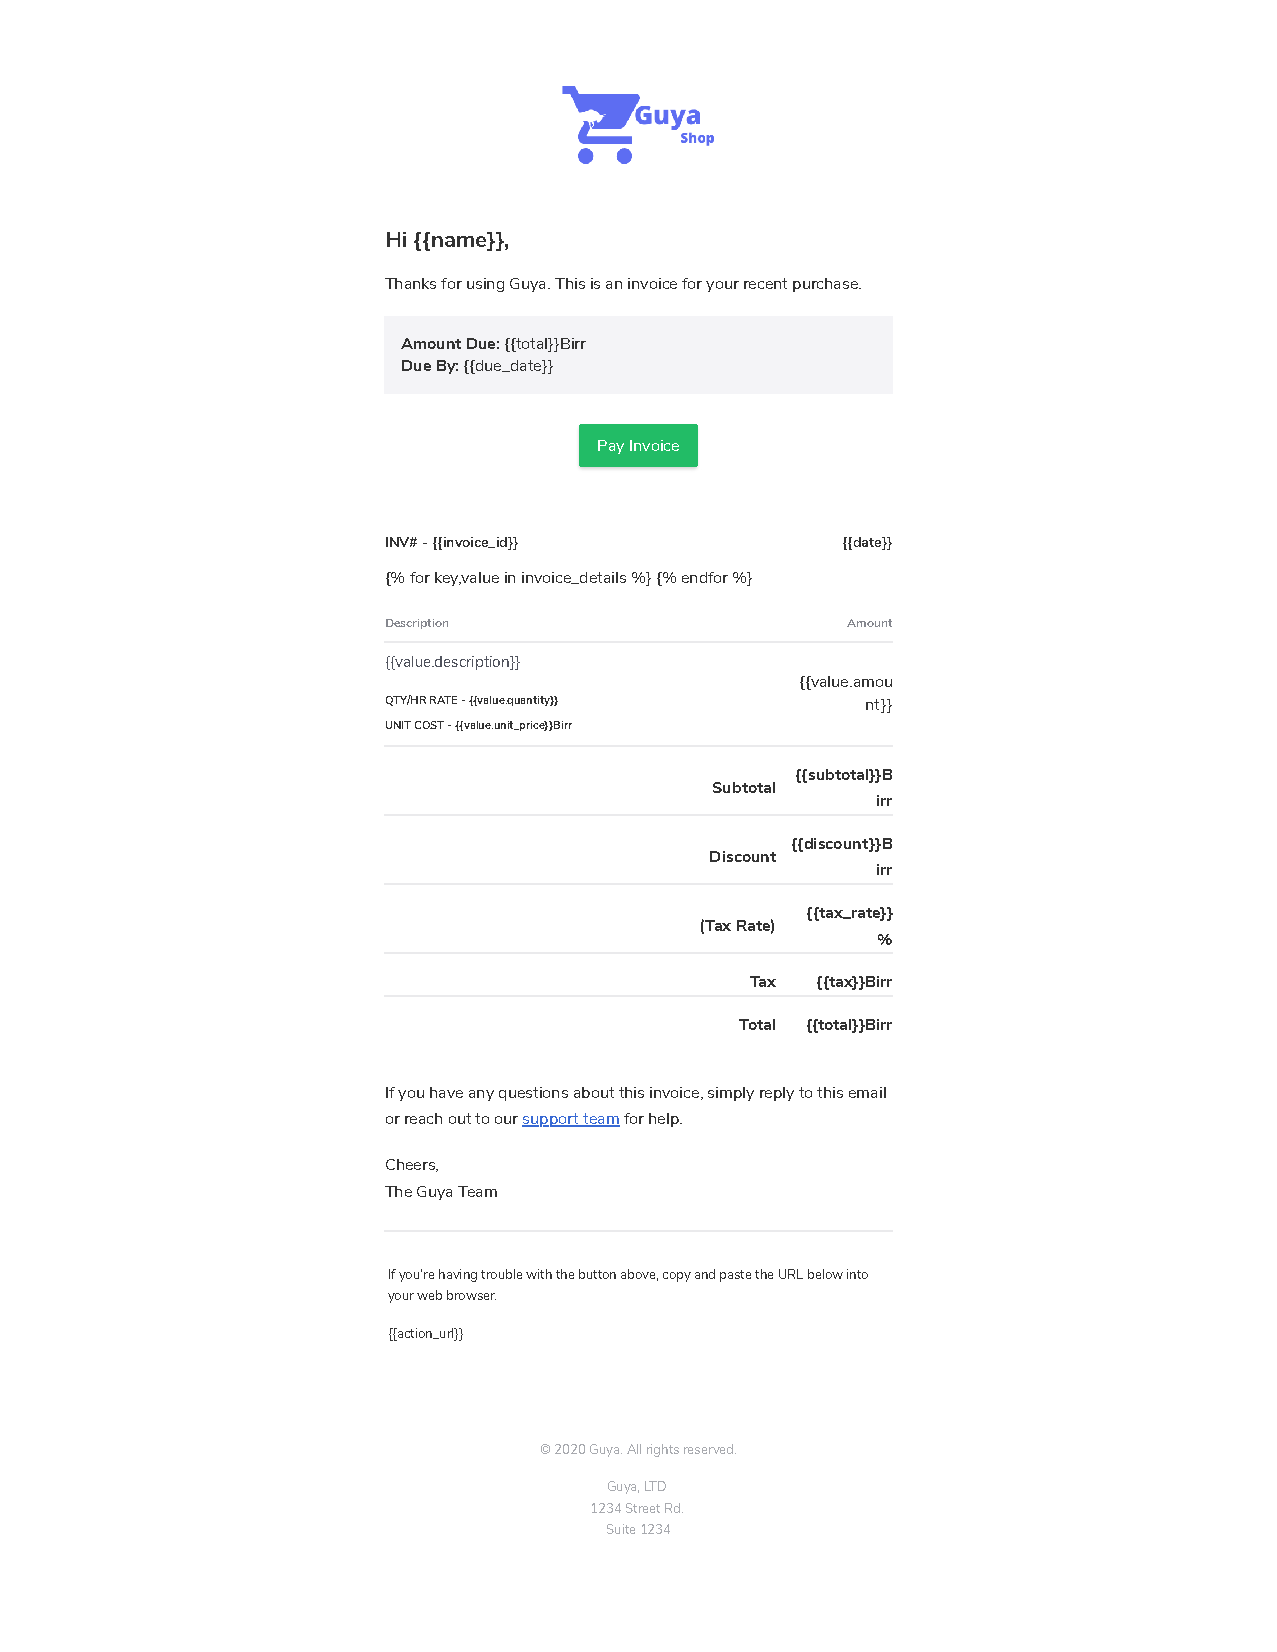
\includepdf[width=20cm, pagecommand={}]{pdf/invoice}
\caption{Invoice Template - Guya E-commerce}
\end{figure}
\clearpage


\begin{figure}[!h]
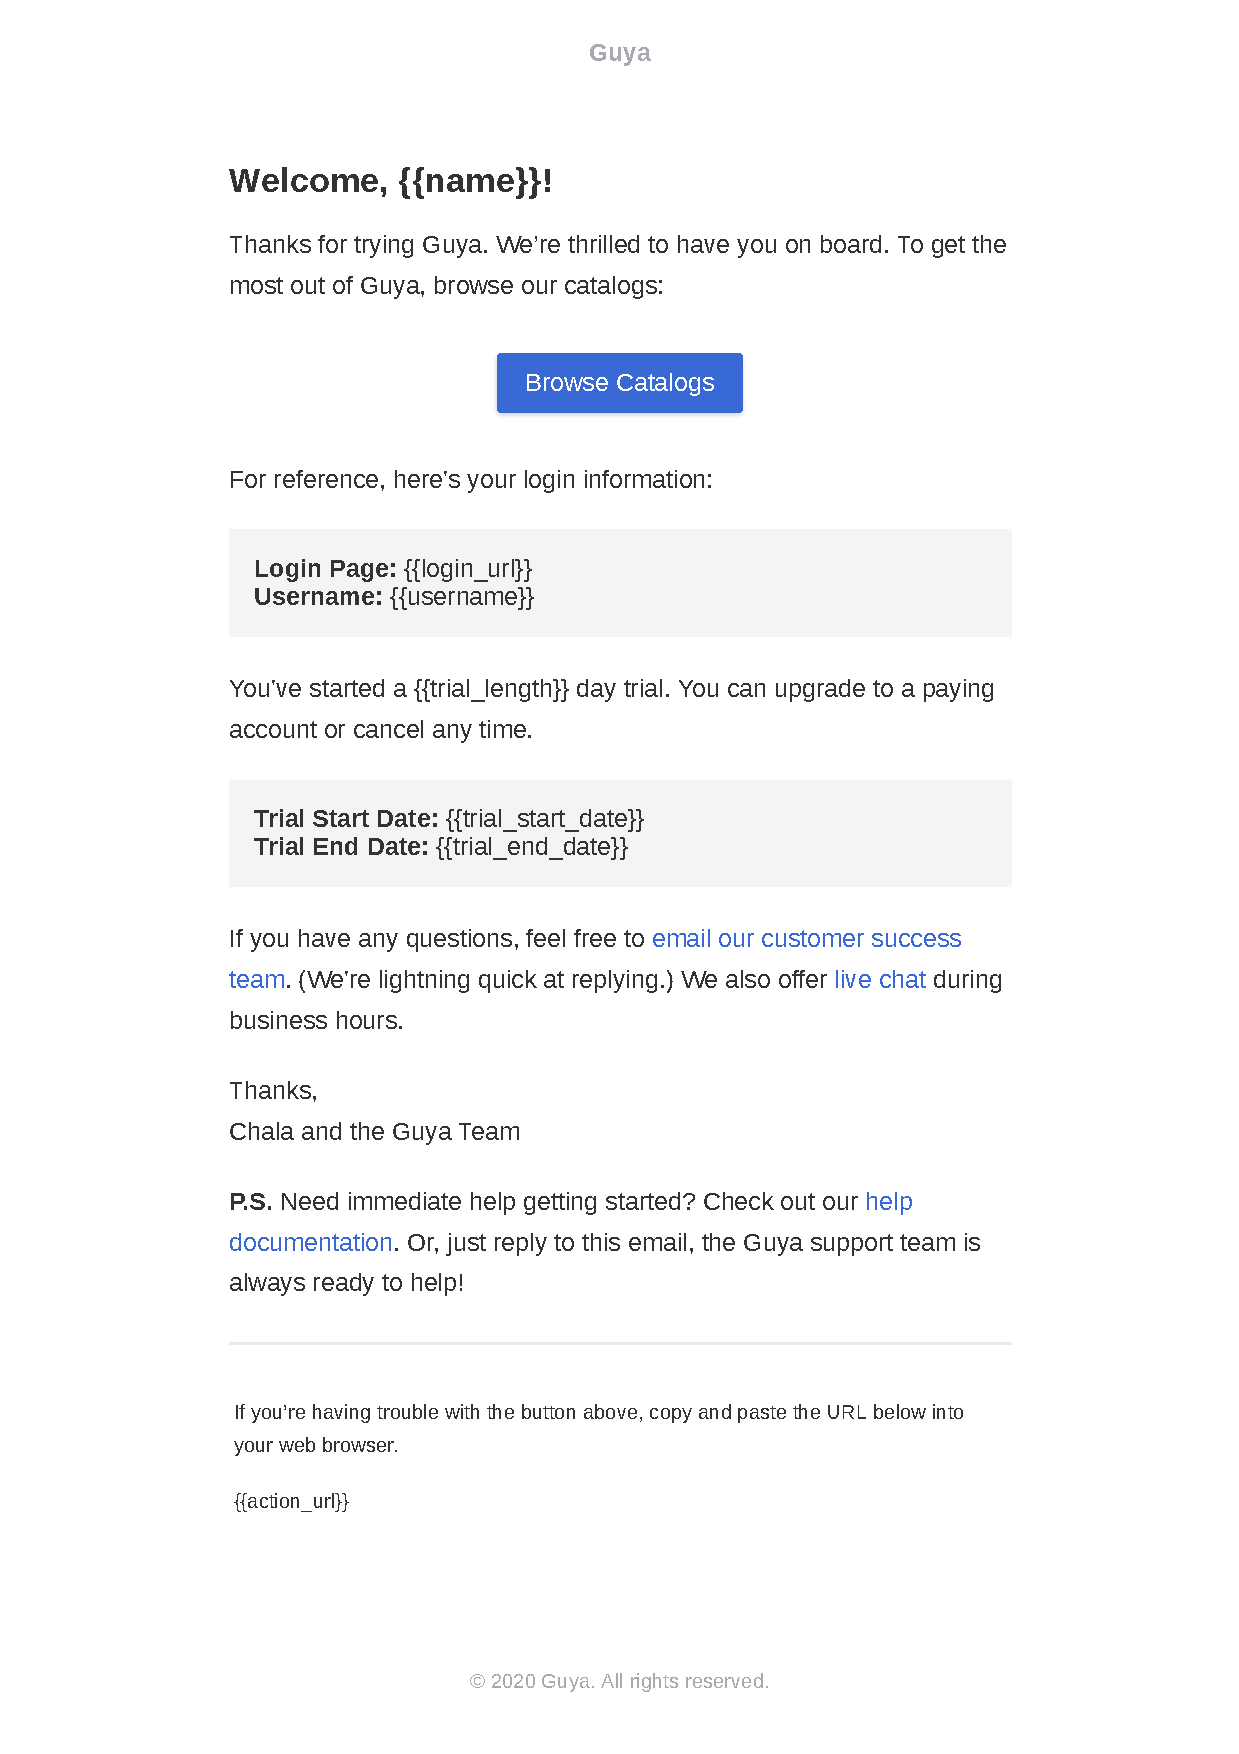
\includepdf[width=15cm, pagecommand={}]{pdf/wellcome}
\caption{Welcome Email Template}
\end{figure}
\clearpage


\begin{figure}[!h]
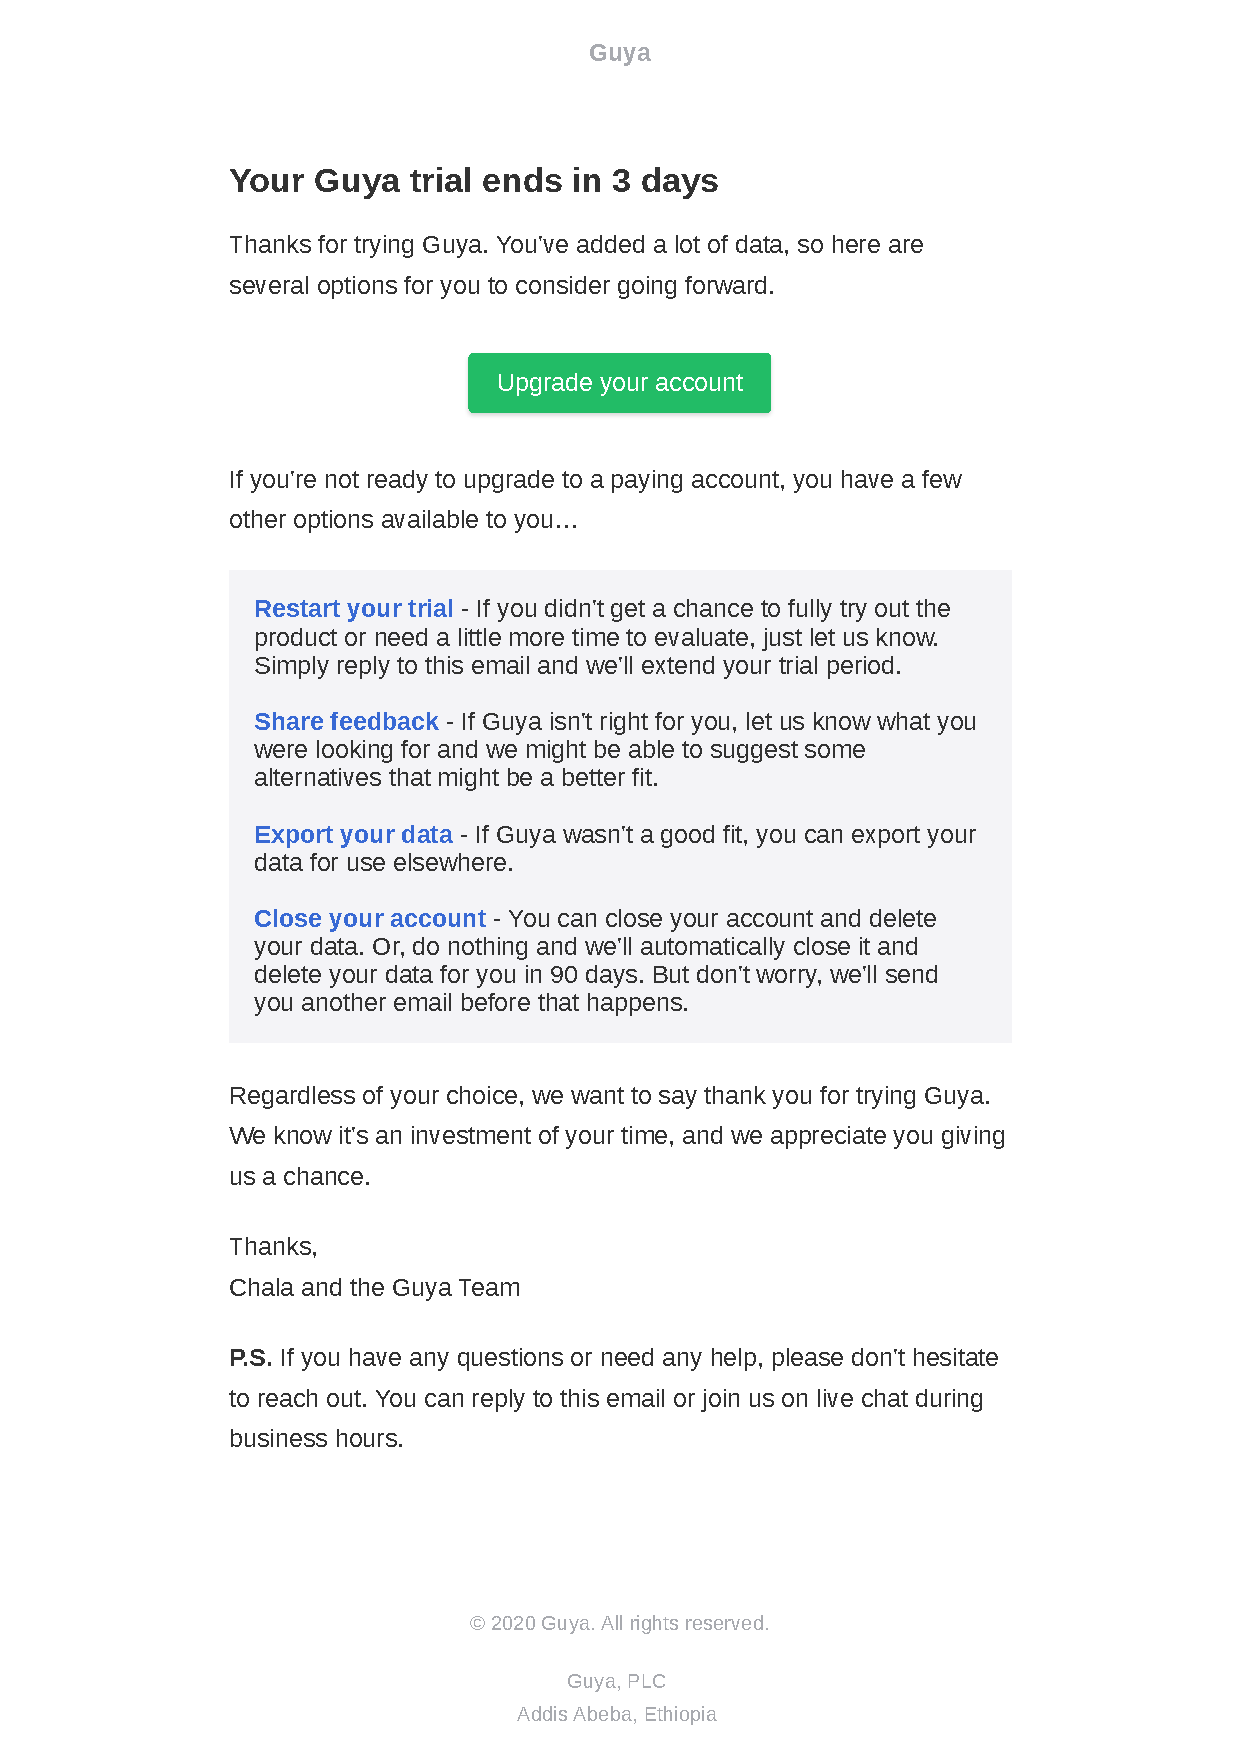
\includepdf[width=15cm, pagecommand={}]{pdf/3day_trail_expire}
\caption{Three days left Trail Template}
\end{figure}
\clearpage


\begin{figure}[!h]
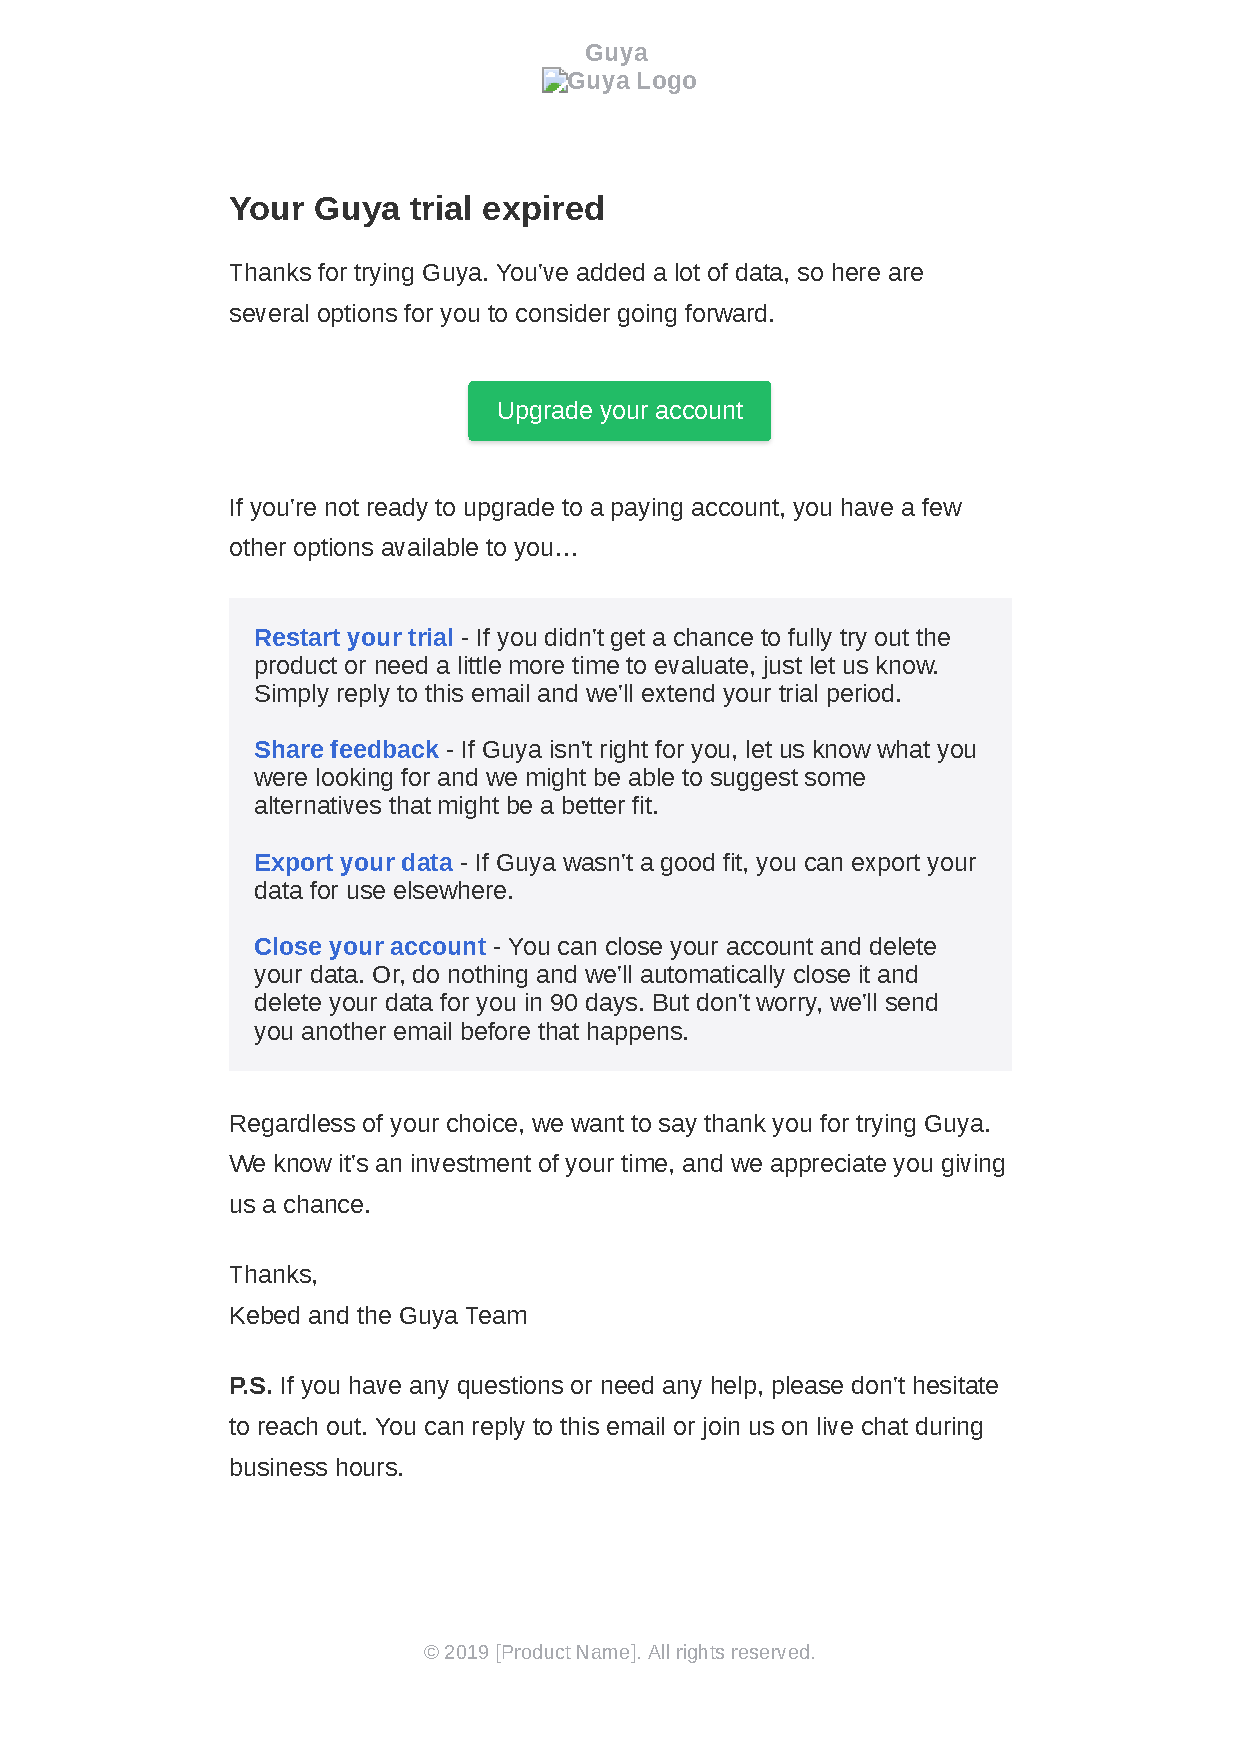
\includepdf[width=15cm,pagecommand={}]{pdf/trial_expired}
\caption{Trial Expired Template}
\end{figure}
\clearpage

\begin{figure}[!h]
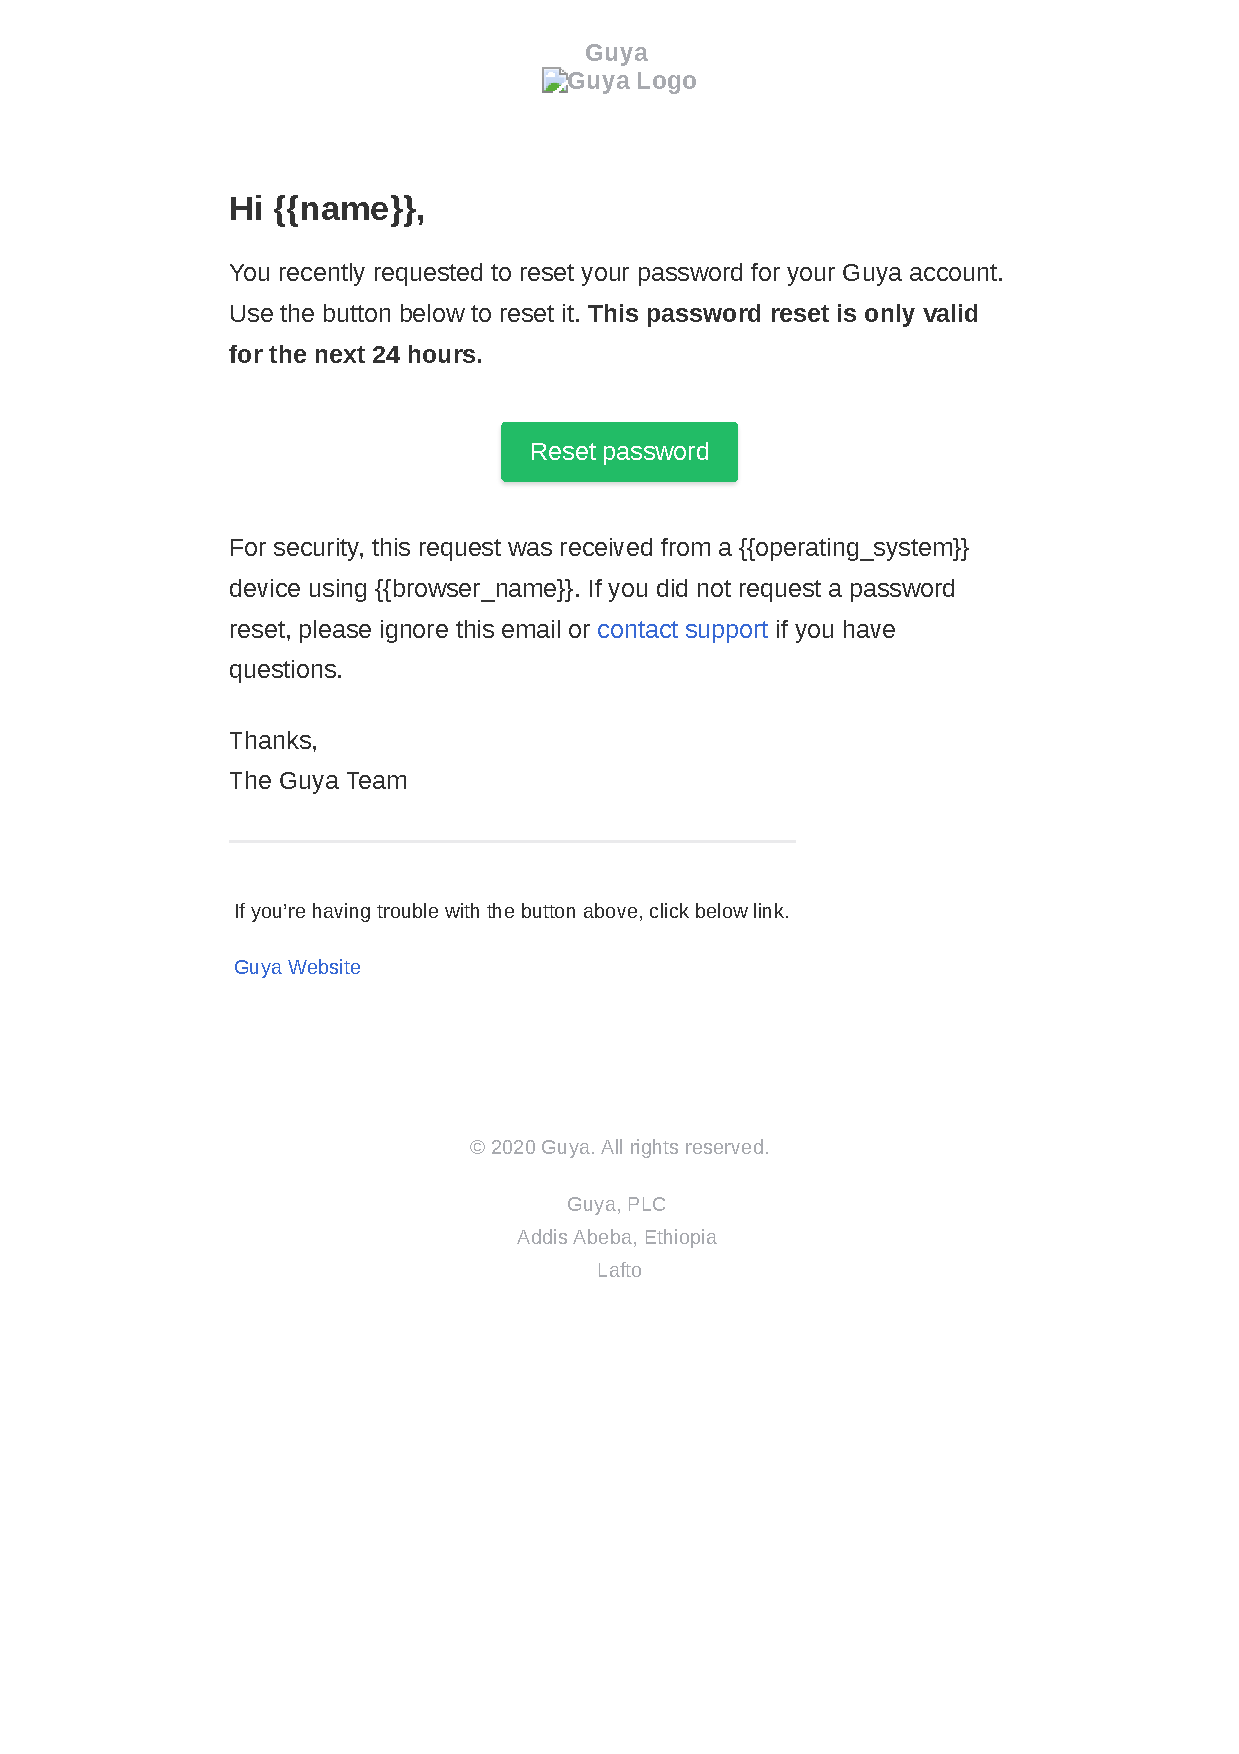
\includepdf[width=15cm, pagecommand={}]{pdf/password_reset}
\caption{Password Reset Template}
\end{figure}
\clearpage

\begin{figure}[!h]
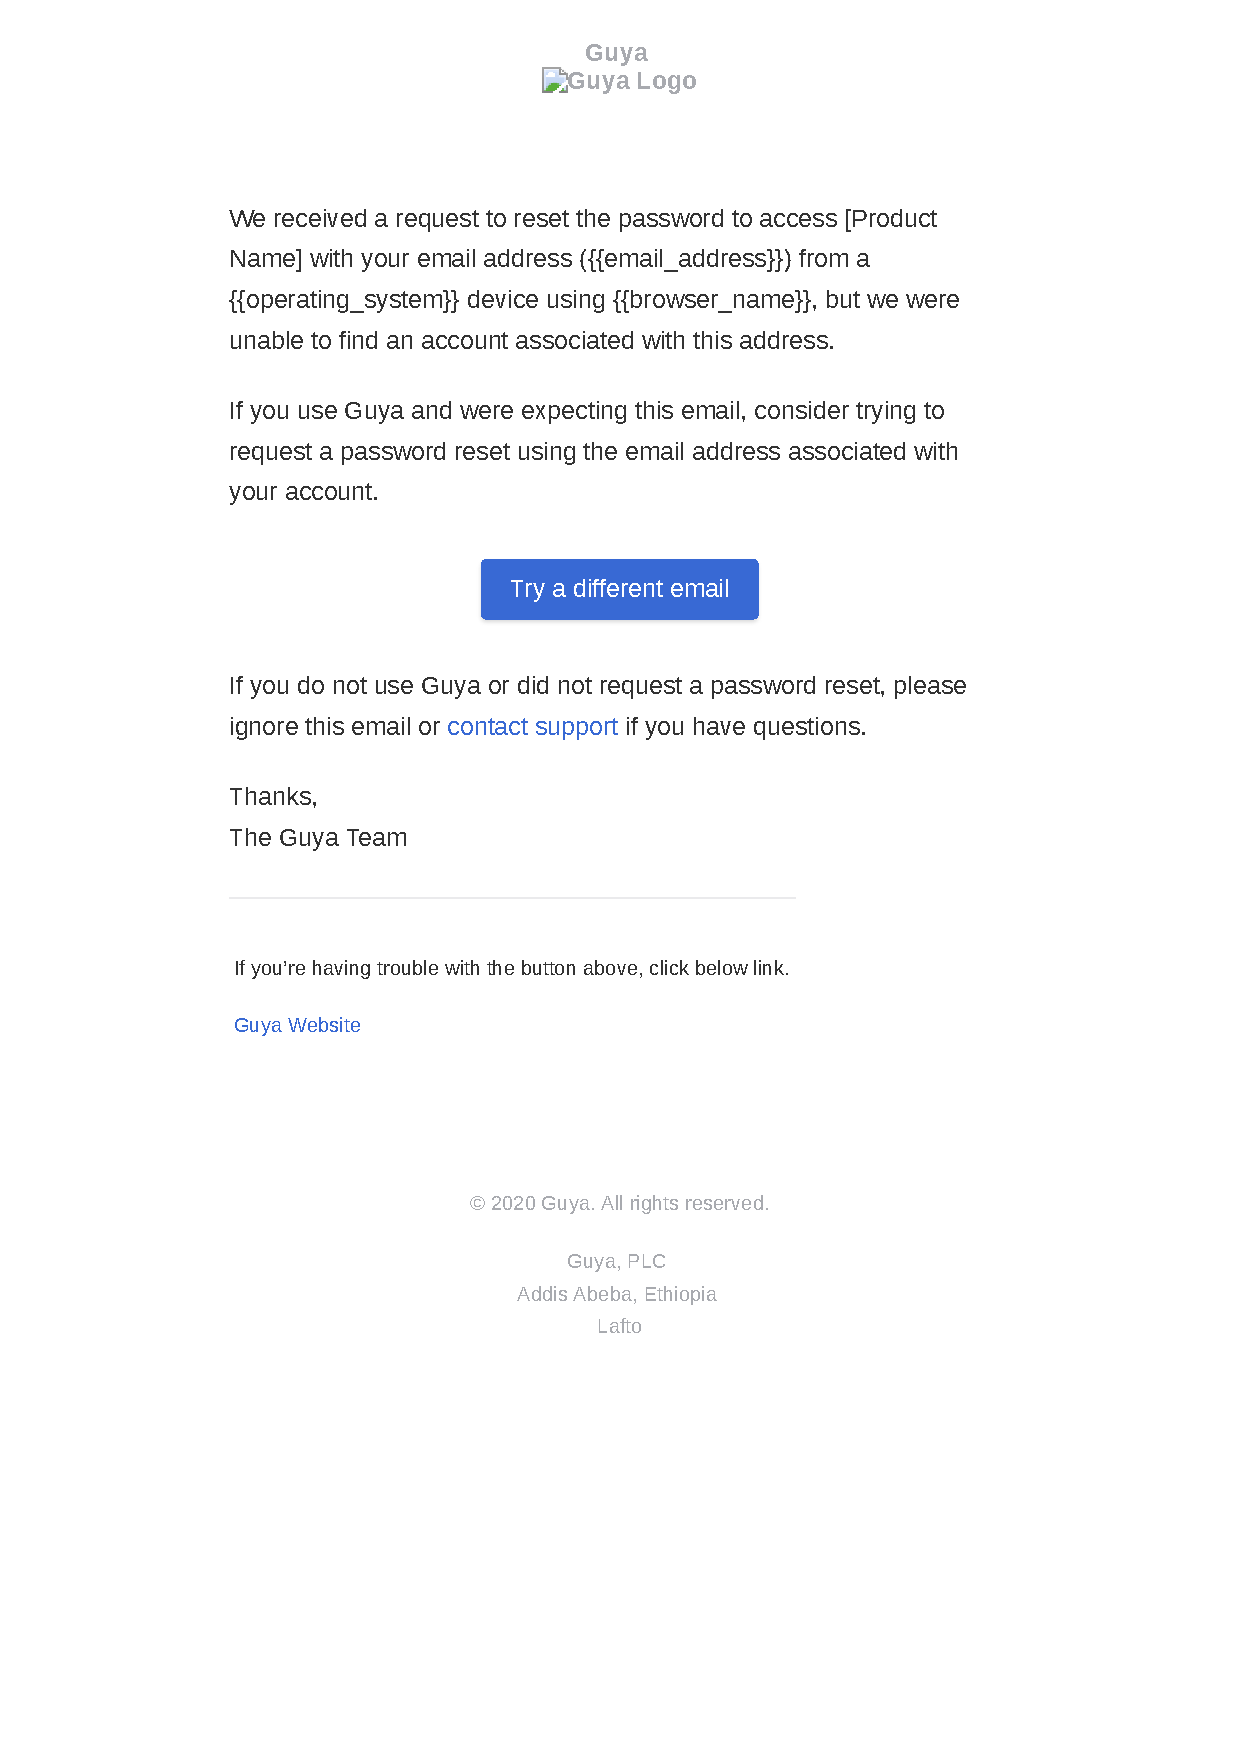
\includepdf[width=15cm, pagecommand={}]{pdf/failed_password_reset}
\caption{Password Reset Failed Template}
\end{figure}
\clearpage


\section{Shipping Label Templates}
Labels are used at every checkpoint of Guya Express shipping process. Starting from pickup point (warehouse or Guya Express location). These labels are used to identify the packages and assign them to correct delivery vans. The labels are designed to be read by both machines and humans.
\subsection{Address Formats}
A post code (also known locally in various English speaking countries throughout the world as a postcode, post code, PIN or ZIP code) is a series of letters or digits or both, sometimes including spaces or punctuation, included in a postal address for the purpose of sorting mail. 
Conversion is done using post code references listed in Appendix C.

\begin{figure}[!h]
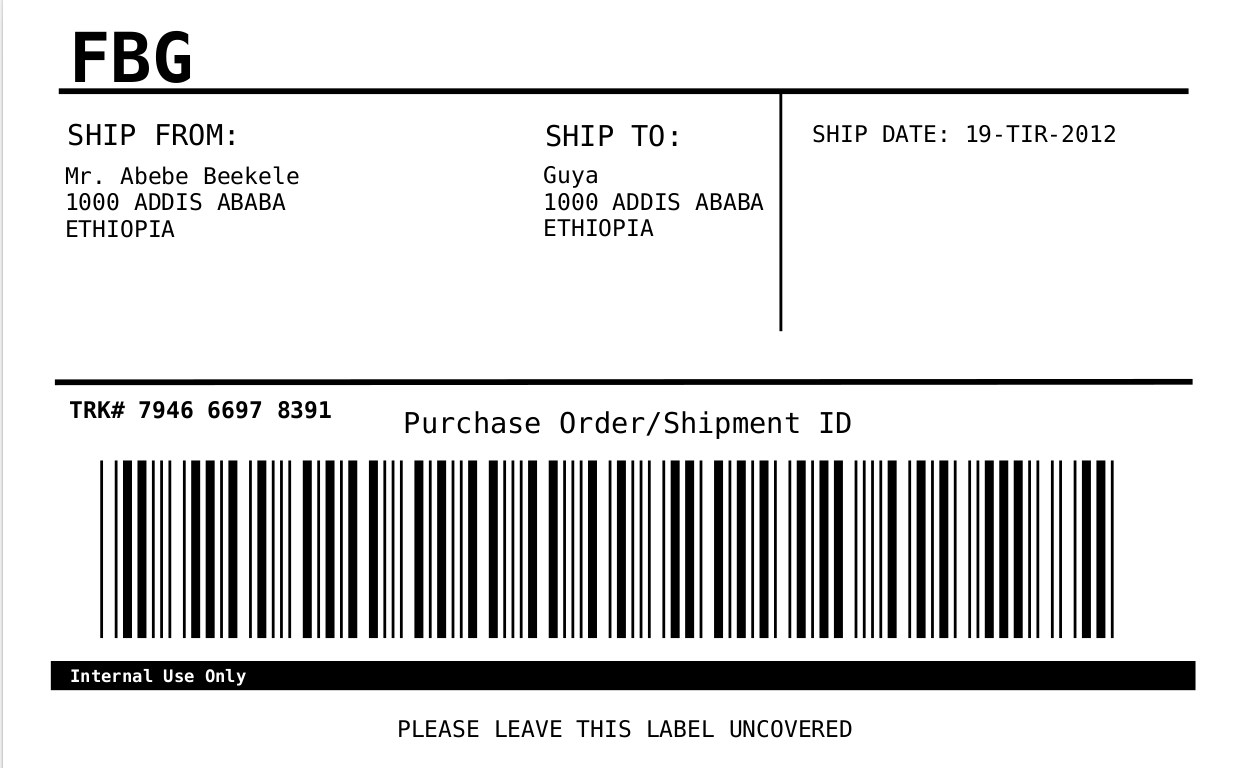
\includegraphics[height=10cm,, keepaspectratio]{images/fpg_shipping}
\caption{Fulfillment Shipping Label template}
\end{figure}
\clearpage

\begin{figure}[!h]
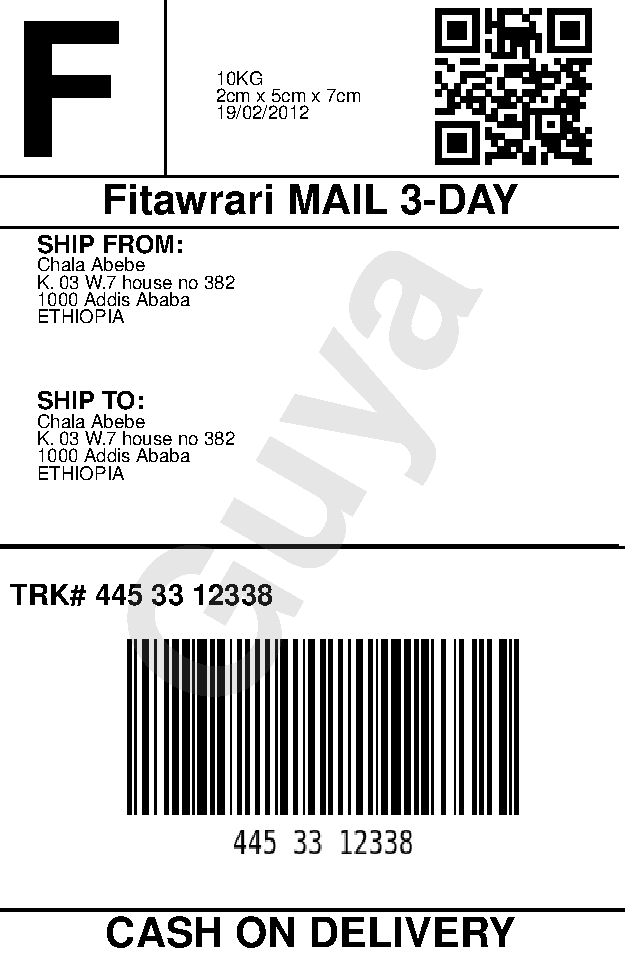
\includegraphics[height=22cm,, keepaspectratio]{images/shipping_label}
\caption{Shipping Label template}
\end{figure}
\clearpage


\section{System Architecture}
\subsection{Component Diagram}
In component diagram we depicts a simplified version of the Component diagram.
Each UML Component describes a microservice, thus component’s name maps one-
to-one with the name of the microservice. Additionally. We have also highlighted
relations among microservices by means of UML Usage relations, i.e. the dashed
arrows labeled with <<use>>.

\begin{figure}[!h]
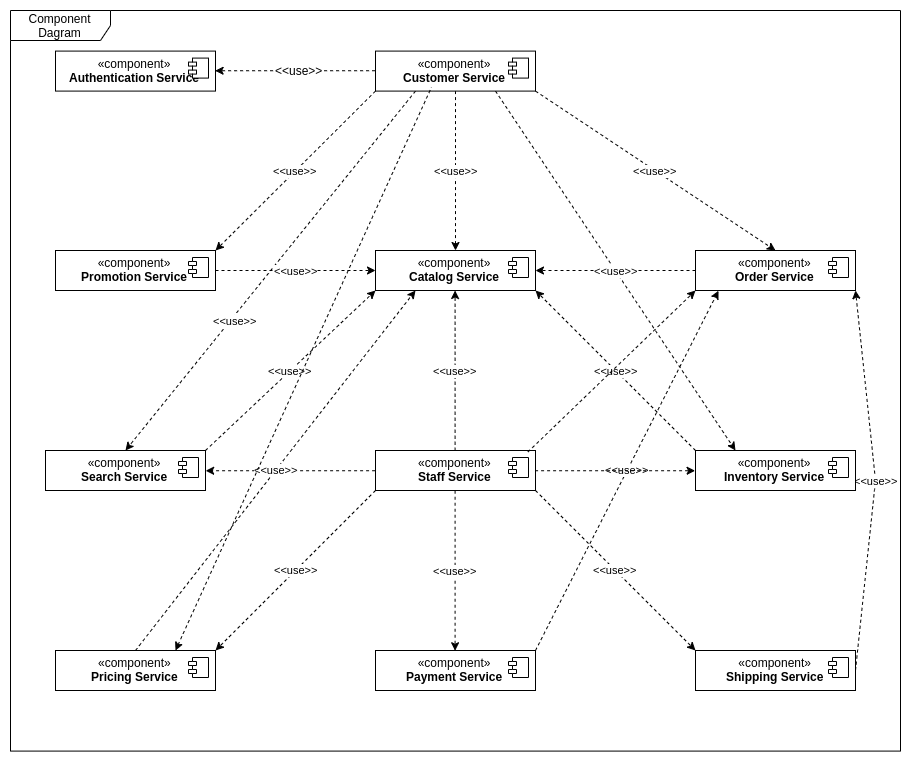
\includegraphics[height=12cm,, keepaspectratio]{images/shop_component_diagram}
\caption{Component Diagram - Guya E-commerce}
\end{figure}

\begin{figure}[!h]
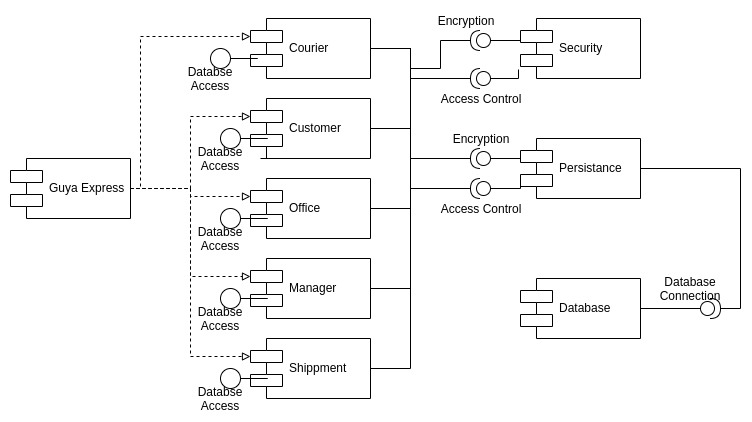
\includegraphics[height=10cm,, keepaspectratio]{images/xpress_component_diagram}
\caption{Component Diagram - Guya E-commerce}
\end{figure}
\clearpage

\subsection{Deployment Diagram}
\begin{figure}[!h]
\hspace{-2cm}
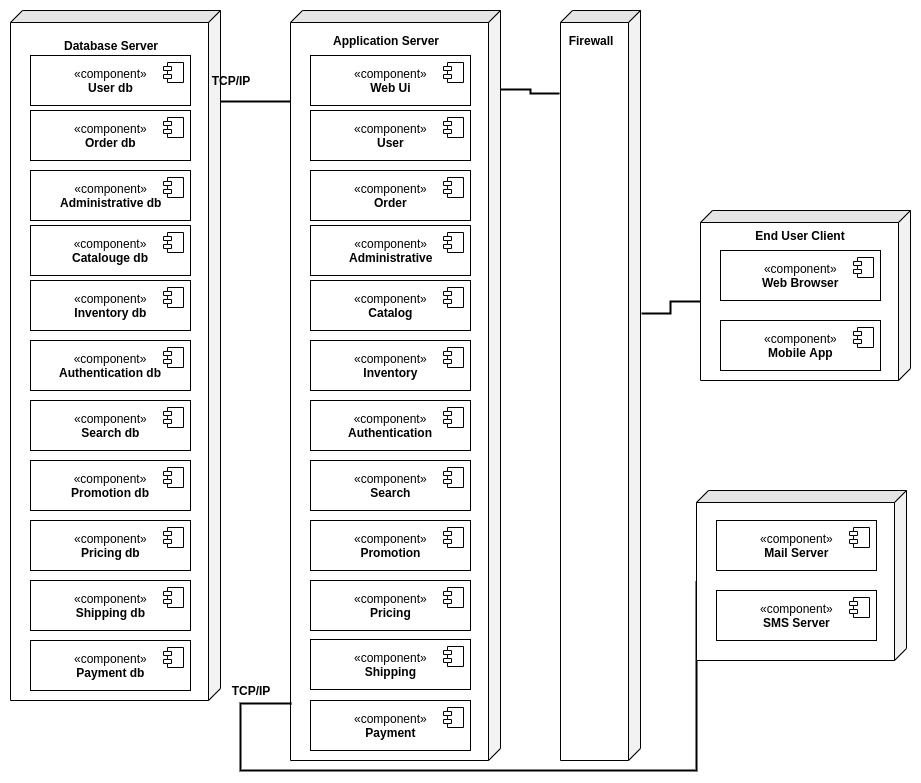
\includegraphics[height=23cm, width=20cm, keepaspectratio]{usecases/shop_deployment_diagram.png}
\caption{Deployment Diagram - Guya E-commerce}
\end{figure}

\begin{figure}[!h]
\hspace{-2cm}
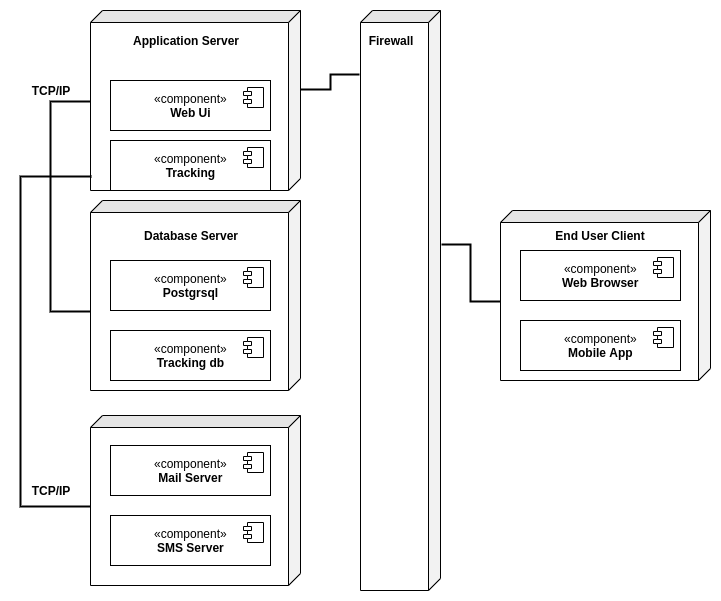
\includegraphics[height=17cm,, keepaspectratio]{images/xpress_deployment_diagram}
\caption{Deployment Diagram - Guya Express}
\end{figure}
\clearpage

\subsection{Network Diagram}
A network diagram is a visual representation of network architecture. It maps out
the structure of a network with a varity of different symbols and line connections.
It is the ideal way to share the layout of a network because the visual presentation
makes it easier for users to understand how items are connected.

\begin{figure}[!h]
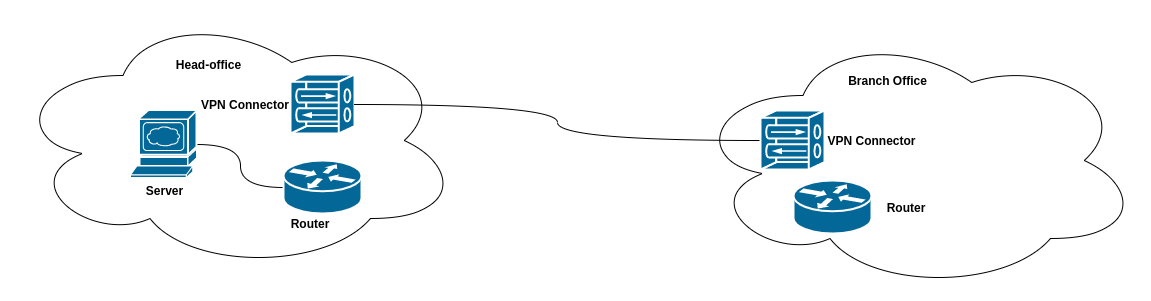
\includegraphics[width=17cm]{images/network_diagram}
\caption{Network Diagram - Guya E-commerce and Express}
\end{figure}
\clearpage


%\subsection{System Physical Architecture}
% three tire system 	
  
%\subsection{System Logical Architecture}
% MVC(Model view controller architecute)	
  
%\subsection{Description of Used Technologies}

%\subsubsection{Docker}
%\subsubsection{Docker Compose}
%\subsubsection{ReactJs}
%\subsubsection{ELK Stack}
%\paragraph{Logstash}
%\paragraph{Elastic Search}
%\paragraph{kibana}
%\subsubsection{Kong Api Gateway}
%\subsubsection{Konga}
%\subsubsection{Sass Css}
%\subsubsection{Openmap}
%\subsubsection{Makefile}
%\subsubsection{Typescript}
%\subsubsection{Webpack}
%\subsubsection{Bit.dev}
%\subsubsection{Storybook}
%\subsubsection{PatternLab}
%\subsubsection{Jade}
%\subsubsection{SQLAlchemy}

%\subsubsection{Handlebars.js}

%\begin{figure}
%\center
%
\includegraphics[keepaspectratio, width=120px]{images/handlebarsjs.png}
%\caption{handlebars.js logo.}
%\end{figure}

%Handlebars is the web template system used in this project to manage client-side templates. It is a JavaScript implementation of the platform-independent Mustache project, that allows to render input data in a template using a very clean syntax. Mustache has a so-called logic-less. template syntax because there are no explicit control flow statements, all needed logic comes exclusively from the data in the form of booleans, arrays or lambdas\footnote{Lambda is an anonymous function, meaning that it is not bound to any kind of identifier.} .On the contrary Handlebars templates are compiled, allowing to define helpers to reuse code for presentation. It also comes with built-in helpers to control the default flow of the template, such as loops or conditional statements. Handlebars comes also with better support for paths
%to access the data. In short, this solution makes easier to implement templates than Mustache while still keeping logic separated from presentation. There is another project, Dust.js, with the same strong points as Handlebars and with useful additional features like template composition. Apparently is a better choice but the project has been abandoned for two years, maybe the reason why Handlebars has the largest community. During the last year LinkedIn has been contributing actively to a separated Dust.js project that
%the company is using for its website [Bas12]. Regardless it has been considered that Handlebars is a safer option, since the additional features are not indispensable for this project.
